\documentclass[a4paper, 11pt]{article}
\usepackage{graphicx}
\usepackage{amsmath}
\usepackage{multicol}
\usepackage{fancyvrb}

\title{Operating Systems \\ Practical Assignment}
\author{Eduardo Freitas Fernandes}
\date{2025}

\begin{document}


\maketitle

\tableofcontents

\newpage

\section{Overview}

In this practical assignment, it's requested to implement a program that simulates the \textbf{communication} between a server and a client. The client has a set of \textbf{requests} to send to the server, and the server processes the request and sends the result to the client. The context of the requests is about \textbf{metadata} relative to documents stored locally on the machine.

The presented implementation uses system calls like \texttt{mkfifo()} and \texttt{open()} to establish the communication between server and client, \texttt{fork()} and \texttt{exec()} variants to consult data in the indexed files, and some others.

The program stores this metadata in a \textbf{file} (disk) and some in \textbf{memory} (cache). It's possible to choose the size of the \textbf{cache} and the \textbf{eviction policy} to use. I've developed some \textbf{Bash scripts} to test and analyse the impact of different cache sizes and types.


\section{Architecture} \label{sec:architecture}

This program is organized in two main parts, the \textbf{client} and the \textbf{server}. The \textbf{client} view is smaller and simpler, given that it only defines the request specified by the user and receives and shows the response given by the server. The \textbf{server} component of this program is more interesting and bigger, since it has to manage client-server communication, memory and disk operations. In the next \textbf{two subsections} I will make a \textbf{detailed} description of those two parts. The program was built upon the following modules:

\begin{multicols}{2}
\begin{itemize}
    \item \texttt{dclient}
    \item \texttt{dserver}
    \item \texttt{client\_ops}
    \item \texttt{server\_ops}
    \item \texttt{defs}
    \item \texttt{document}
    \item \texttt{free\_list}
    \item \texttt{index\_table}
    \item \texttt{cache}
    \item \texttt{fifo\_cache}
    \item \texttt{rand\_cache}
    \item \texttt{lru\_cache}
    \item \texttt{utils}
\end{itemize}
\end{multicols}

\noindent The \texttt{utils} module is a general purpose module, used to implement functions needed in other modules but do not fit it's context. The \texttt{document} module is used to store the metadata relative to the real document, stored locally.

\begin{Verbatim}[xleftmargin=2em]
typedef struct document {
    char title[TITLE_SIZE];
    char authors[AUTHORS_SIZE];
    char year[YEAR_SIZE];
    char path[PATH_SIZE];
} Document;
\end{Verbatim}

\noindent The \texttt{defs} module (it's just a header file) defines \textbf{macros} essential for all the other modules, like the name of the file to store the metadata, sizes for the metadata and a \texttt{struct} relative to a \textbf{Request}.

\begin{Verbatim}[xleftmargin=2em]
typedef struct {
    pid_t client;
    Operation operation;
    char title[TITLE_SIZE];
    char authors[AUTHORS_SIZE];
    char year[YEAR_SIZE];
    char path[PATH_SIZE];
} Request;
\end{Verbatim}

\noindent The \texttt{client} field indicates the process identifier of the process (client) that sent the request. The \texttt{operation} field indicates the type of request to perform, the available values will be presented ahead. The remaining fields are used to transport the arguments necessary to execute the request.

\begin{figure}[h]
    \centering
    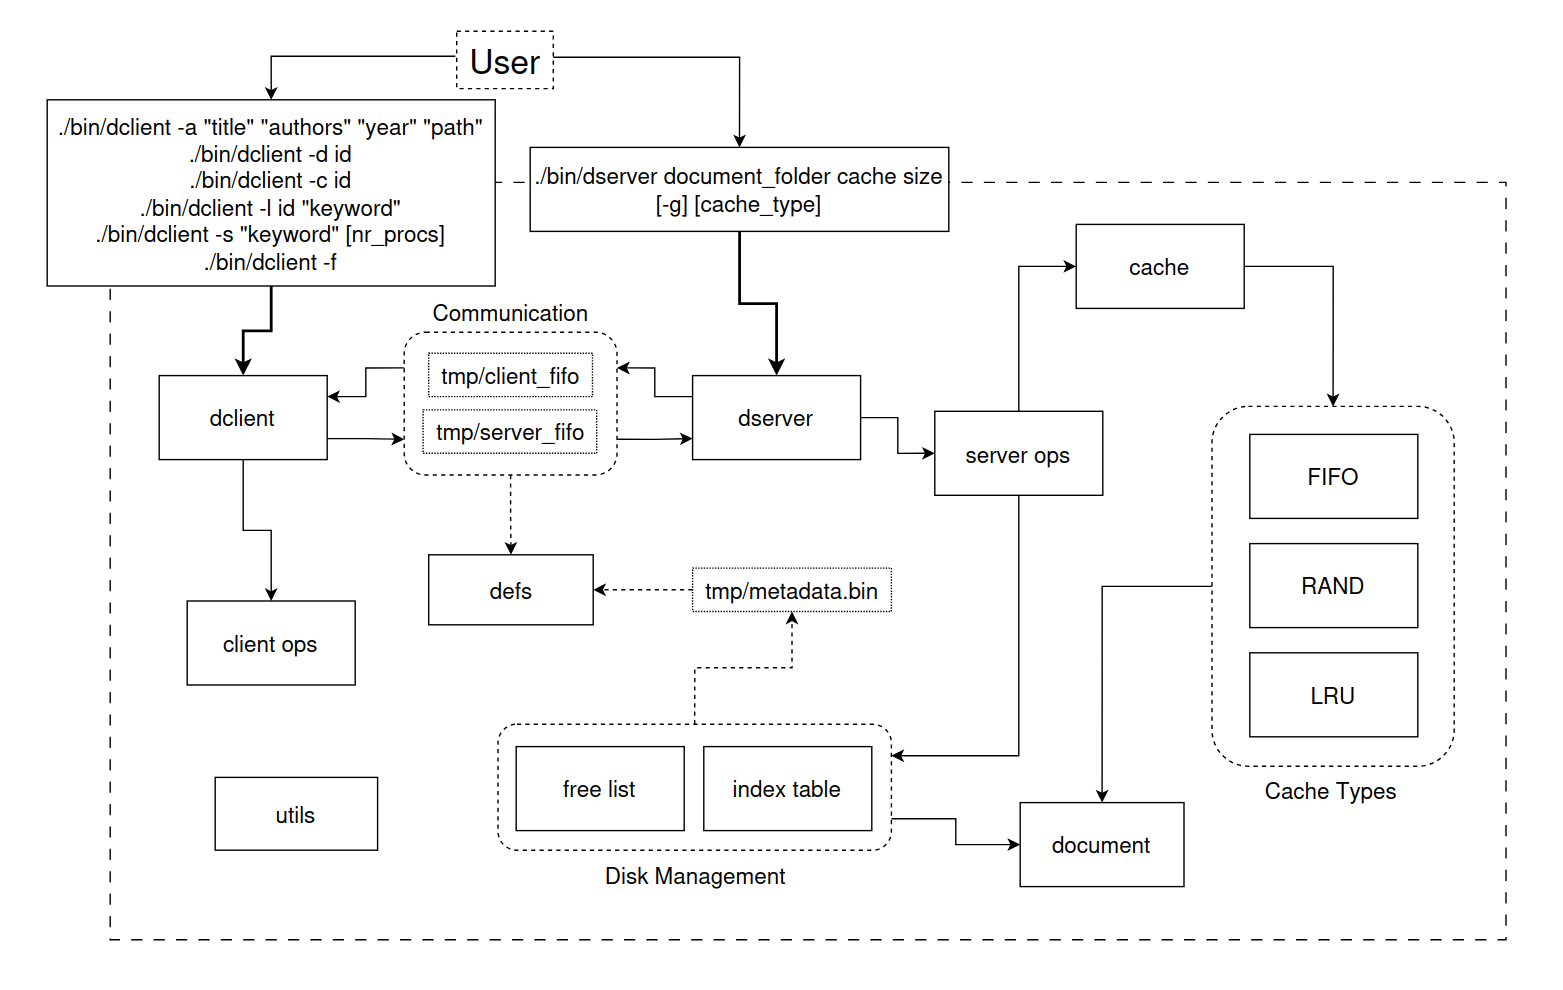
\includegraphics[width=1\linewidth]{report-diagram.png}
    \caption{Program Diagram}
    \label{fig:diagram}
\end{figure}

\noindent In Figure \ref{fig:diagram} we can see the usage of every module and how they interlink with each other. The user starts by turning on the server. The client them sends a request to the server through \texttt{SERVER\_FIFO}. The indexed metadata is being kept in the \texttt{STORAGE\_FILE} file and managed by the \textbf{Free List} and \textbf{Index Table}. The \texttt{server\_ops} module uses these two data structures and the \textbf{Cache} to answer the requests. The server then sends a reply through \texttt{CLIENT\_FIFO} to the user.

\subsection{Client}

The modules that belong to this program component are:

\begin{itemize}
    \item \texttt{dclient}: main program that the user uses to send requests, receive replies and show it's content.
    \item \texttt{client\_ops}: this module ensures the request sent by the user is valid and takes care of the output for the user.
\end{itemize}

\noindent The user calls the \texttt{dclient} binary with a flag (e.g. -a, -d, -s) and the necessary arguments for that operation. Through the \texttt{client\_ops} module, the program validates the given arguments, i.e. checks if the number of arguments is correct. The client creates a pipe with name (FIFO) (e.g. \texttt{client\_fifo\_24}), that will be used to receive the response sent by the server. This FIFO is unique and the only process that will read data from it is the client who created it. After this, the client opens the FIFO created by the server to send a request. This FIFO is shared by all the clients, so every request is sent by this FIFO named \texttt{SERVER\_FIFO}. The client sends the request using the system call \texttt{write()}, and depending on the operation, opens the private FIFO and, using the system call \texttt{read()}, receives the response from the server. Once again, the \texttt{client\_ops} module helps the client and shows the response.


\subsection{Server}

The modules that belong to this program component are:

\begin{itemize}
    \item \texttt{dserver}: main program that the user uses to start the server, receive requests and do operations.
    \item \texttt{server\_ops}: module that contains all the server operations, whether it's request processing, disk or memory management.
    \item \texttt{free\_list}: data structure used to store available document identifiers
    \item \texttt{index\_table}: data structure used to indicate which documents are valid
\end{itemize}

\noindent The \textbf{cache} modules are managed by the server, so they should be included in this listing; however, the cache is a topic I want to discuss separately.

\noindent The server is the main piece of the program. It's the first binary to be executed. The server starts by creating the main channel \texttt{SERVER\_FIFO} to receive requests from clients. Then creates (or uploads) the necessary data structures to run and enters a loop to receive the request sent by other processes. After receiving a \texttt{SHUTDOWN} message, it frees all the data structures and records the necessary information in disk.

\subsubsection{Operations}

The available request types are:

\begin{itemize}
    \item \texttt{INDEX}: index metadata relative to a file
    \item \texttt{REMOVE}: remove an index of metadata
    \item \texttt{CONSULT}: retrieve the metadata relative to a file
    \item \texttt{COUNT\_WORD}: count the number of lines a keyword occurs in a document
    \item \texttt{LIST\_WORD}: list the documents that contain a keyword
    \item \texttt{SHUTDOWN}: shut down the server
    \item \texttt{KILL}: tell the server a child process finished its execution
\end{itemize}

\noindent To \textbf{index} metadata about a document, the server records a \texttt{Document} \texttt{struct} in disk (\texttt{STORAGE\_FILE}) with the help of the \textbf{Free List} and \textbf{Index Table}. After this, the metadata is also recorded in \textbf{memory} (Cache). To \textbf{remove} an indexation, the server marks the document as invalid in the \textbf{Index Table}, and reuses the document identifier through the \textbf{Free List}. These operations are done by the original server process, so other clients have to wait for these operations to finish.\\

\noindent \textbf{NOTE}: The following operations are consultations, meaning they do not modify the stored metadata. Therefore, clients should not have to wait for others performing the same operations, as specified in the project brief. However, implementing a cache is also required. To ensure the cache content persists between operations, it must be maintained by a single process (since each process has its own instance). To balance both requirements, I decided that the \texttt{CONSULT} and \texttt{COUNT\_WORD} operations will be handled by the server, meaning clients will have to wait in these cases. The \texttt{LIST\_WORD} operation, on the other hand, is performed by a child process, primarily because it iterates over all documents and is more time-consuming, while the other two operations are very fast as they access only a single document.\\

\noindent The \texttt{CONSULT} operation is meant to show the metadata indexed relative to a document. The server uses the \textbf{Index Table} to see if the document is indexed, then goes to \texttt{STORAGE\_FILE} (or cache) and reads the metadata and sends it to the client. The \texttt{COUNT\_WORD} operation is similar, only with some additional tasks. The server reads the metadata, grabs the filename and runs \texttt{grep -c} to count the number of lines the keyword occurs, and sends the response. \texttt{COUNT\_WORD} task uses an \textbf{anonymous pipe} (created with the system call \texttt{pipe()}) to send the count to server.\\

\noindent The \texttt{LIST\_WORD} operation is done by another process, so that the server can do other tasks and other clients don't have to wait. The default number of processes to execute this task is 1. Through the \textbf{Index Table} we can obtain an array with the valid document identifiers. We then divide the identifiers by the number of processes, and each one takes care of a chunk. This operation uses a single \textbf{anonymous pipe} to communicate with the child processes, charged of each chunk. If a process finds a document with the keyword, it sends the identifier to the parent process, that stores the ID. An important thing to say is that the processes access the \texttt{STORAGE\_FILE}, but they don't share the offset (they each use the system call \texttt{open()} to avoid this). After creating all the necessary processes, the parent process enters a loop and reads all the document IDs sent in the anonymous pipe. After this is done, it waits (system call \texttt{wait()}) for every child process.\\

\noindent \textbf{NOTE}: Each of the operations described above send a \textbf{response} to the client, so they either create a child process and he does it, or the current process does it (\texttt{COUNT\_WORD} and \texttt{LIST\_WORD} cases).\\

\noindent The \texttt{SHUTDOWN} command tells the server to turn off. The client does not receive an answer. The server records the necessary data in disk (Free List and Index Table) and free the allocated space for the data structures.\\

\noindent The \texttt{KILL} instruction is used by the child processes of the server. This operation tells the server that a process has finished it's work and it's in zombie mode, waiting for someone to get its return value. This trick allows the server to block in a single place, in the FIFO named \texttt{SERVER\_FIFO}.

\subsubsection{Disk Management}

The disk management is done by two data structures, the \textbf{Free List} and \textbf{Index Table}. A document identifier is an integer, and it's used to determine the position in which the metadata is kept in \texttt{STORAGE\_FILE}. The \texttt{Document struct} has a static size, and the metadata is stored sequentially inside the file, so we only need the identifier to access it.\\

\noindent The \textbf{Index Table} is as follows:

\begin{Verbatim}[xleftmargin=2em]
typedef struct index_table {
    unsigned capacity;
    unsigned count;
    char *table;
} Index_Table;
\end{Verbatim}

\noindent It's a simple dynamic array of characters. This table is used as an array of \textbf{valid bits}. Each \texttt{char} holds 8 bits, each one relative to a document. If a bit has the value 0, it means is not valid, does not exist. This approach allows very \textbf{fast lookups} and the \textbf{space usage} is very low. A lookup is done like so: \texttt{(table[id / 8] >> (id \% 8)) \& 1}.\\

\noindent The \textbf{Free List} has the following structure:

\begin{Verbatim}[xleftmargin=2em]
struct link {
    int id;
    struct link *next;
};

typedef struct free_list {
    struct link *head;
    unsigned size;
} Free_List;
\end{Verbatim}

\noindent This data structure is used to prevent \textbf{internal fragmentation}, when removing indexes. The metadata is stored sequentially, so when an index is removed, the program stores the document identifier in a \textbf{stack}, and when the next indexation happens, it \textbf{reuses} the stored document identifier. This is a simple stack, implemented with a linked list.\\

\noindent Both of these data structures are \textbf{persisted} in a file (\texttt{CONTROL\_FILE}), because when the server is turned off, it's necessary to know which documents are valid or not.

\subsection{Cache}

The modules used for the cache implementation are:

\begin{itemize}
    \item \texttt{cache}
    \item \texttt{fifo\_cache}
    \item \texttt{rand\_cache}
    \item \texttt{lru\_cache}
\end{itemize}

\noindent The \textbf{Cache} module holds a \textbf{polymorphic} cache container structure. It stores function pointers to the selected cache functions. This is necessary because there are multiple cache implementations, this approach allows, if necessary, an expansion of the cache implementations.\\

\noindent The cache is an \textbf{independent} layer of this program. If no cache is used, the server accesses disk through the index table and free list, otherwise, the server requests a document from cache, if there is a \textbf{hit}, returns the document, if there is a \textbf{miss}, it accesses the disk through the same process, and then returns the document.\\

\noindent All the implementations have 4 components in common: an array of \texttt{Documents} to store the metadata, an array of identifiers (integers) relatives to the documents, the size of the arrays and a file descriptor (\texttt{source}), used to retrieve metadata from disk, in a cache miss.\\

\noindent To optimize the \texttt{LIST\_WORD} operation, every cache implements a \textbf{prefetching} technique. If I search for document 30 and there is a cache miss, the cache goes to disk and brings documents 30 to 37. This saves some time, because in the \texttt{-s} task we know that if we search for document \texttt{i}, the next search will be \texttt{i+1}.

\subsubsection{FIFO Eviction Policy}

The FIFO cache has the following structure:

\begin{Verbatim}[xleftmargin=2em]
typedef struct fifo {
    Document *documents;
    int *identifiers;
    int back;
    int size;
    int source;
} FIFO_Cache;
\end{Verbatim}

\noindent The \texttt{back} field is used to indicate the next position to insert metadata. Once the cache is full it will start to remove the metadata added at first, following a First-In-First-Out idea.

\subsubsection{RAND Eviction Policy}

The RAND cache has the following structure:

\begin{Verbatim}[xleftmargin=2em]
typedef struct rand {
    Document *documents;
    int *identifiers;
    int size;
    int source;
} RAND_Cache;
\end{Verbatim}

\noindent This implementation is the simplest. When adding a set of documents, select a \textbf{random position} to place them.

\subsubsection{LRU Eviction Policy}

The LRU cache has the following structure:

\begin{Verbatim}[xleftmargin=2em]
typedef struct lru {
    Document *documents;
    int *identifiers;
    char *ref_bits;
    int size;
    int source;
    int back;
} LRU_Cache;
\end{Verbatim}

\noindent This cache implementation tries approximating a \textbf{Least Recently Used} eviction policy. The \texttt{ref\_bits} field is an array of characters that indicates if the position is "valuable", in other words, indicates if the position was used recently. When adding metadata, search for free positions, then positions with reference bits to 0.


\section{Usage}

To build and run the program, you must follow these instructions in the specified order. First of all, run \texttt{make} to build the object files and create the necessary folders. After this operation, there should be two binary files (\texttt{dserver} and \texttt{dclient}) in the \texttt{bin} directory.


\subsection{DServer}

The server is the first binary to be executed, otherwise the program will not run properly. The server must be initiated with the following structure:

\begin{verbatim}
./bin/dserver document_folder cache_size [-g] [cache_type]
\end{verbatim}

\begin{itemize}
    \item \texttt{document\_folder}: directory in which the documents are stored locally
    \item \texttt{cache\_size}: maximum number of entries of metadata to be kept in memory
    \item \texttt{-g}: turn off debugging messages (optional)
    \item \texttt{cache\_type}: select the type of eviction policy for the cache. This argument is optional. If no type is given, cache is not used.
\end{itemize}

\noindent After executing this command, it's safe to send requests to the server, through the client.


\subsection{DClient}

After starting up the server, the user can execute the \texttt{dclient} binary and send requests to the program server. There is no need to show the usage of the \texttt{dclient} command, the usage is explained in the project brief.


\section{Critical Analysis}

The last part of this assignment we are asked to analyse the performance of using multiple processes to optimize the list documents operation and to compare the multiple cache eviction policies and its different sizes. In the \texttt{scripts} directory you may find scripts to test the performance of the program. The results shown in the next two sub sections were obtained in my machine:

\begin{itemize}
    \item \textbf{Model}:
    \item \textbf{Processor}:
    \item \textbf{Memory}:
    \item \textbf{Operating System}:
\end{itemize}

\subsection{List Documents results}


\subsection{Cache results}


\end{document}
